%%
%% Automatically generated file from DocOnce source
%% (https://github.com/hplgit/doconce/)
%%
%%
% #ifdef PTEX2TEX_EXPLANATION
%%
%% The file follows the ptex2tex extended LaTeX format, see
%% ptex2tex: http://code.google.com/p/ptex2tex/
%%
%% Run
%%      ptex2tex myfile
%% or
%%      doconce ptex2tex myfile
%%
%% to turn myfile.p.tex into an ordinary LaTeX file myfile.tex.
%% (The ptex2tex program: http://code.google.com/p/ptex2tex)
%% Many preprocess options can be added to ptex2tex or doconce ptex2tex
%%
%%      ptex2tex -DMINTED myfile
%%      doconce ptex2tex myfile envir=minted
%%
%% ptex2tex will typeset code environments according to a global or local
%% .ptex2tex.cfg configure file. doconce ptex2tex will typeset code
%% according to options on the command line (just type doconce ptex2tex to
%% see examples). If doconce ptex2tex has envir=minted, it enables the
%% minted style without needing -DMINTED.
% #endif

% #define PREAMBLE

% #ifdef PREAMBLE
%-------------------- begin preamble ----------------------

\documentclass[%
oneside,                 % oneside: electronic viewing, twoside: printing
final,                   % draft: marks overfull hboxes, figures with paths
10pt]{article}

\listfiles               % print all files needed to compile this document

\usepackage{relsize,makeidx,color,setspace,amsmath,amsfonts,amssymb}
\usepackage[table]{xcolor}
\usepackage{bm,microtype}

\usepackage[pdftex]{graphicx}

\usepackage[T1]{fontenc}
%\usepackage[latin1]{inputenc}
\usepackage{ucs}
\usepackage[utf8x]{inputenc}

\usepackage{lmodern}         % Latin Modern fonts derived from Computer Modern

% Hyperlinks in PDF:
\definecolor{linkcolor}{rgb}{0,0,0.4}
\usepackage{hyperref}
\hypersetup{
    breaklinks=true,
    colorlinks=true,
    linkcolor=linkcolor,
    urlcolor=linkcolor,
    citecolor=black,
    filecolor=black,
    %filecolor=blue,
    pdfmenubar=true,
    pdftoolbar=true,
    bookmarksdepth=3   % Uncomment (and tweak) for PDF bookmarks with more levels than the TOC
    }
%\hyperbaseurl{}   % hyperlinks are relative to this root

\setcounter{tocdepth}{2}  % number chapter, section, subsection

% Tricks for having figures close to where they are defined:
% 1. define less restrictive rules for where to put figures
\setcounter{topnumber}{2}
\setcounter{bottomnumber}{2}
\setcounter{totalnumber}{4}
\renewcommand{\topfraction}{0.95}
\renewcommand{\bottomfraction}{0.95}
\renewcommand{\textfraction}{0}
\renewcommand{\floatpagefraction}{0.75}
% floatpagefraction must always be less than topfraction!
% 2. ensure all figures are flushed before next section
\usepackage[section]{placeins}
% 3. enable begin{figure}[H] (often leads to ugly pagebreaks)
%\usepackage{float}\restylefloat{figure}

% newcommands for typesetting inline (doconce) comments
\newcommand{\shortinlinecomment}[3]{{\color{red}{\bf #1}: #2}}
\newcommand{\longinlinecomment}[3]{{\color{red}{\bf #1}: #2}}

% prevent orhpans and widows
\clubpenalty = 10000
\widowpenalty = 10000

% --- end of standard preamble for documents ---


% insert custom LaTeX commands...

\raggedbottom
\makeindex

%-------------------- end preamble ----------------------

\begin{document}

% endif for #ifdef PREAMBLE
% #endif


% ------------------- main content ----------------------



% ----------------- title -------------------------

\thispagestyle{empty}

\begin{center}
{\LARGE\bf
\begin{spacing}{1.25}
FFM232, Klassisk fysik och vektorfält - Föreläsningsanteckningar
\end{spacing}
}
\end{center}

% ----------------- author(s) -------------------------

\begin{center}
{\bf \href{{http://fy.chalmers.se/subatom/tsp/}}{Christian Forssén}, Institutionen för fysik, Chalmers, Göteborg, Sverige${}^{}$} \\ [0mm]
\end{center}

\begin{center}
% List of all institutions:
\end{center}
    
% ----------------- end author(s) -------------------------

% --- begin date ---
\begin{center}
Sep 9, 2016
\end{center}
% --- end date ---

\vspace{1cm}


\section{3. Integraler}
Det mesta av detta material förutsätts vara känt från kursen i flervariabelanalys. Vi kommer att repetera
\paragraph{Linje- (kurv-) integraler.}
\begin{itemize}
\item t.ex. $\int_C \vec{F} \cdot d\vec{r}$

\item eller $\int_C \phi \cdot ds$

\item eller ...

\item (integral över en sluten kurva betecknas $\oint_C \vec{F} \cdot d\vec{r}$)
\end{itemize}

\noindent
\paragraph{Ytintegraler.}
\begin{itemize}
\item t.ex. $\int_S \vec{F} \cdot d\vec{S}$

\item eller ...

\item (integral över en sluten yta betecknas $\oint_C \vec{F} \cdot d\vec{S}$)
\end{itemize}

\noindent
% inline figure
\centerline{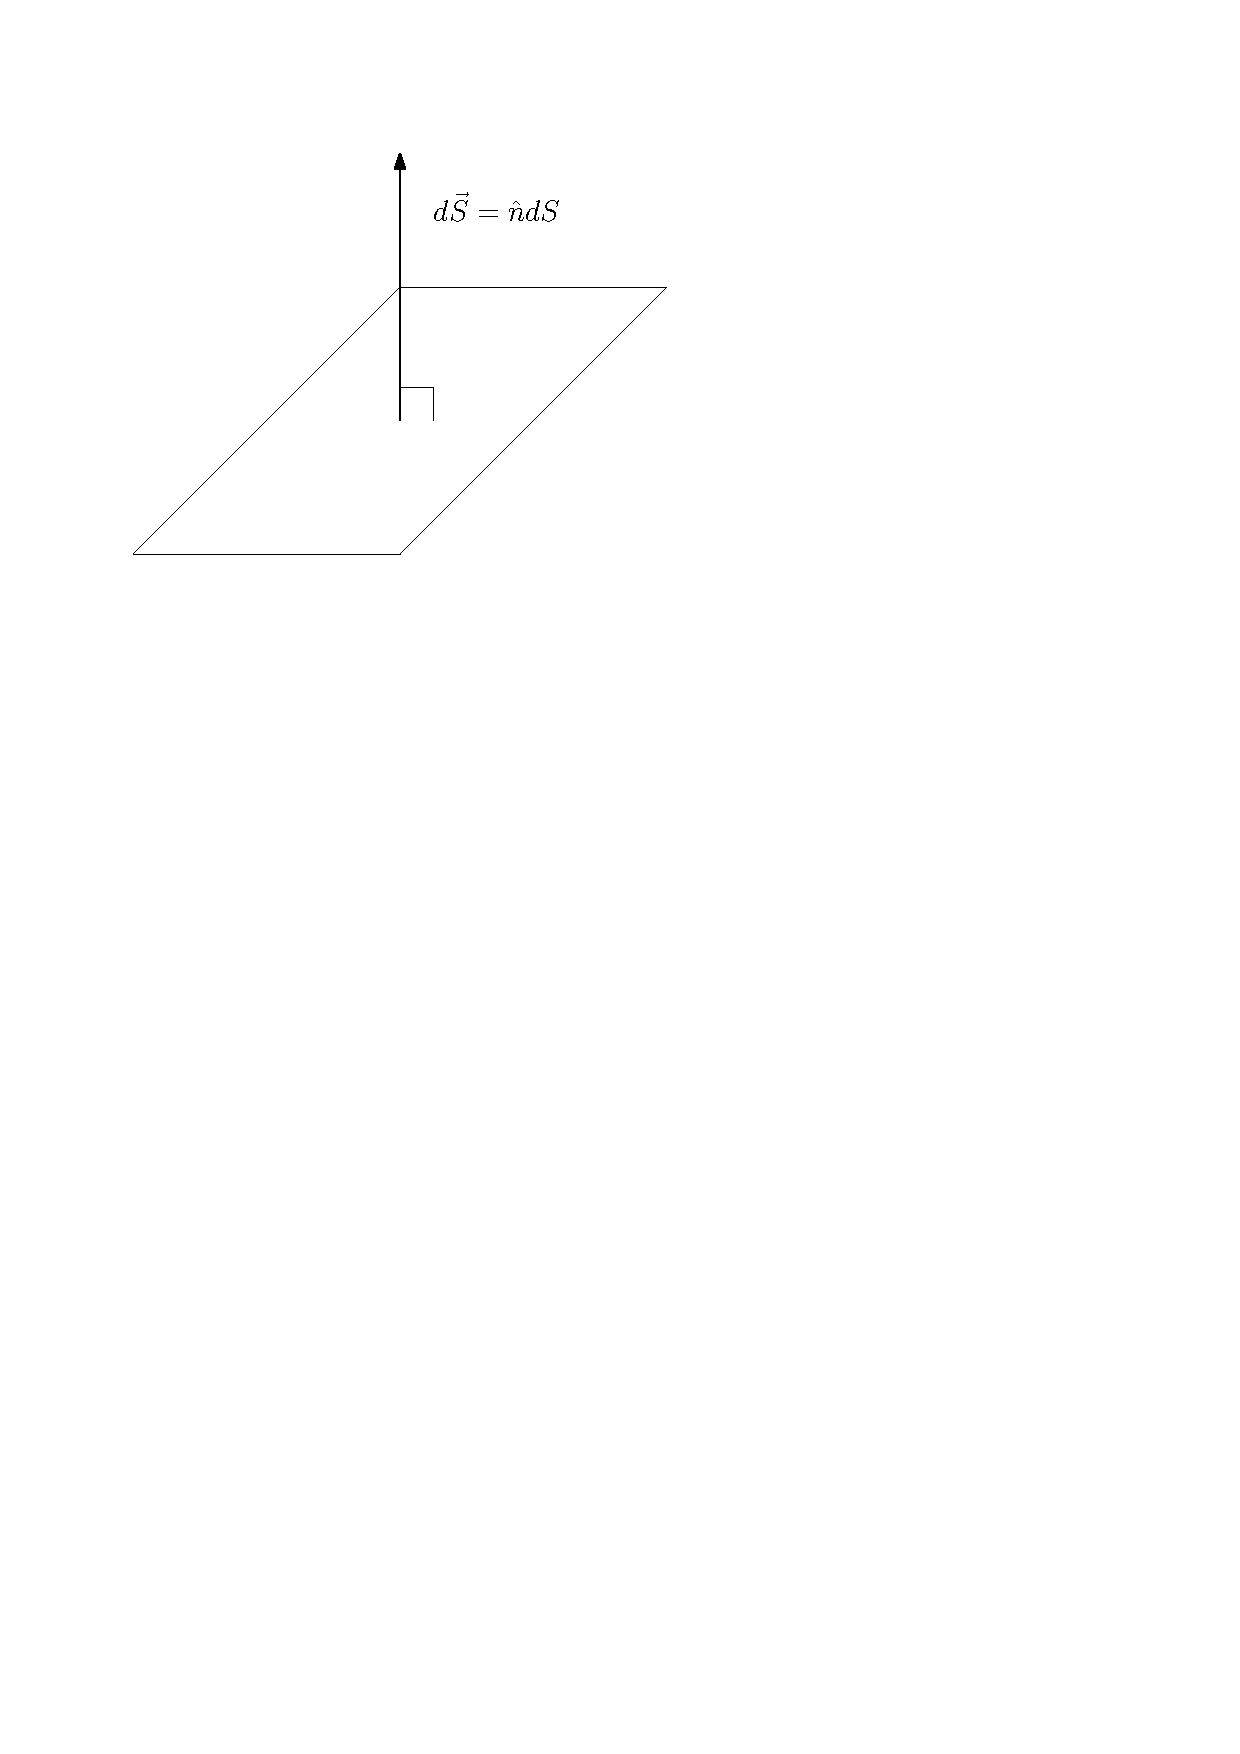
\includegraphics[width=0.4\linewidth]{fig/yta.pdf}}



\paragraph{Volymintegraler.}
\begin{itemize}
\item $\int_V \vec{F} dV$
\end{itemize}

\noindent
\subsection{Parametrisering}
Integralerna kan i allmänhet lösas genom parametrisering. 

\paragraph{Parametrisering av kurvintegraler:}
T.ex. ges en kurva $C$ av $\vec{r}(\tau)$ med $\tau \in [\tau_1,\tau_2]$. Då blir
\begin{equation}
  \int_C \vec{F}\cdot \mbox{d}\vec{r} = \int_{\tau_1}^{\tau_2} \vec{F}
\cdot \frac{\mbox{d}\vec{r}}{\mbox{d}\tau} \mbox{d}\tau,
\end{equation}
och efter att ha beräknat skalärprodukten har vi en helt vanlig endimensionell integral.



% inline figure
\centerline{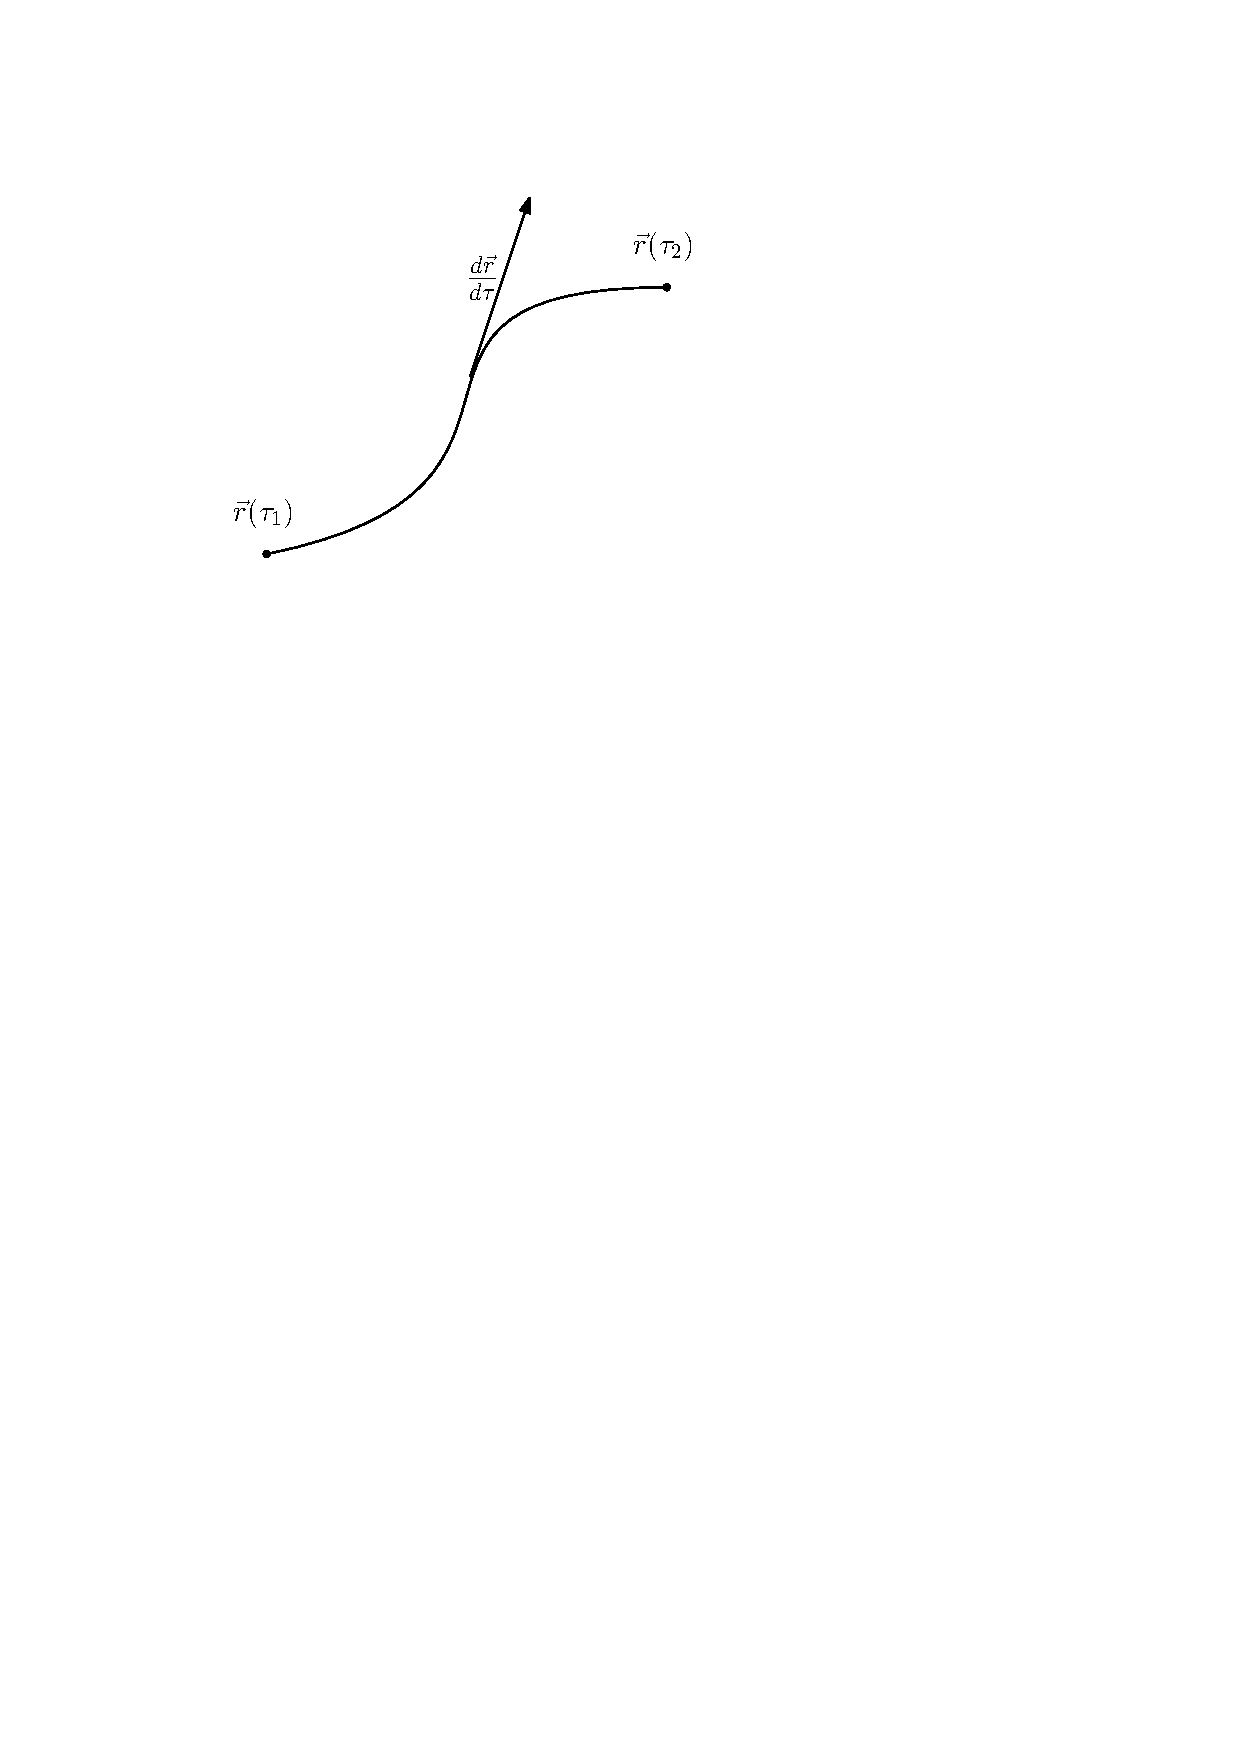
\includegraphics[width=0.4\linewidth]{fig/kurva.pdf}}



\longinlinecomment{Comment 1}{ Lägg här märke till att $d\vec{r}/d\tau$ är en tangentvektor till kurvan $C$.  I princip finns det oändligt många parametriseringar till kurvan $C$, och rent matematiskt spelar det ingen roll vilken man väljer, fast vissa parametriseringar ger snällare räkningar än andra! }{ Lägg här märke till }

Ibland är kurvan $C$ sluten, det vill säga kurvans start- och slutpunkt sammanfaller. 



% inline figure
\centerline{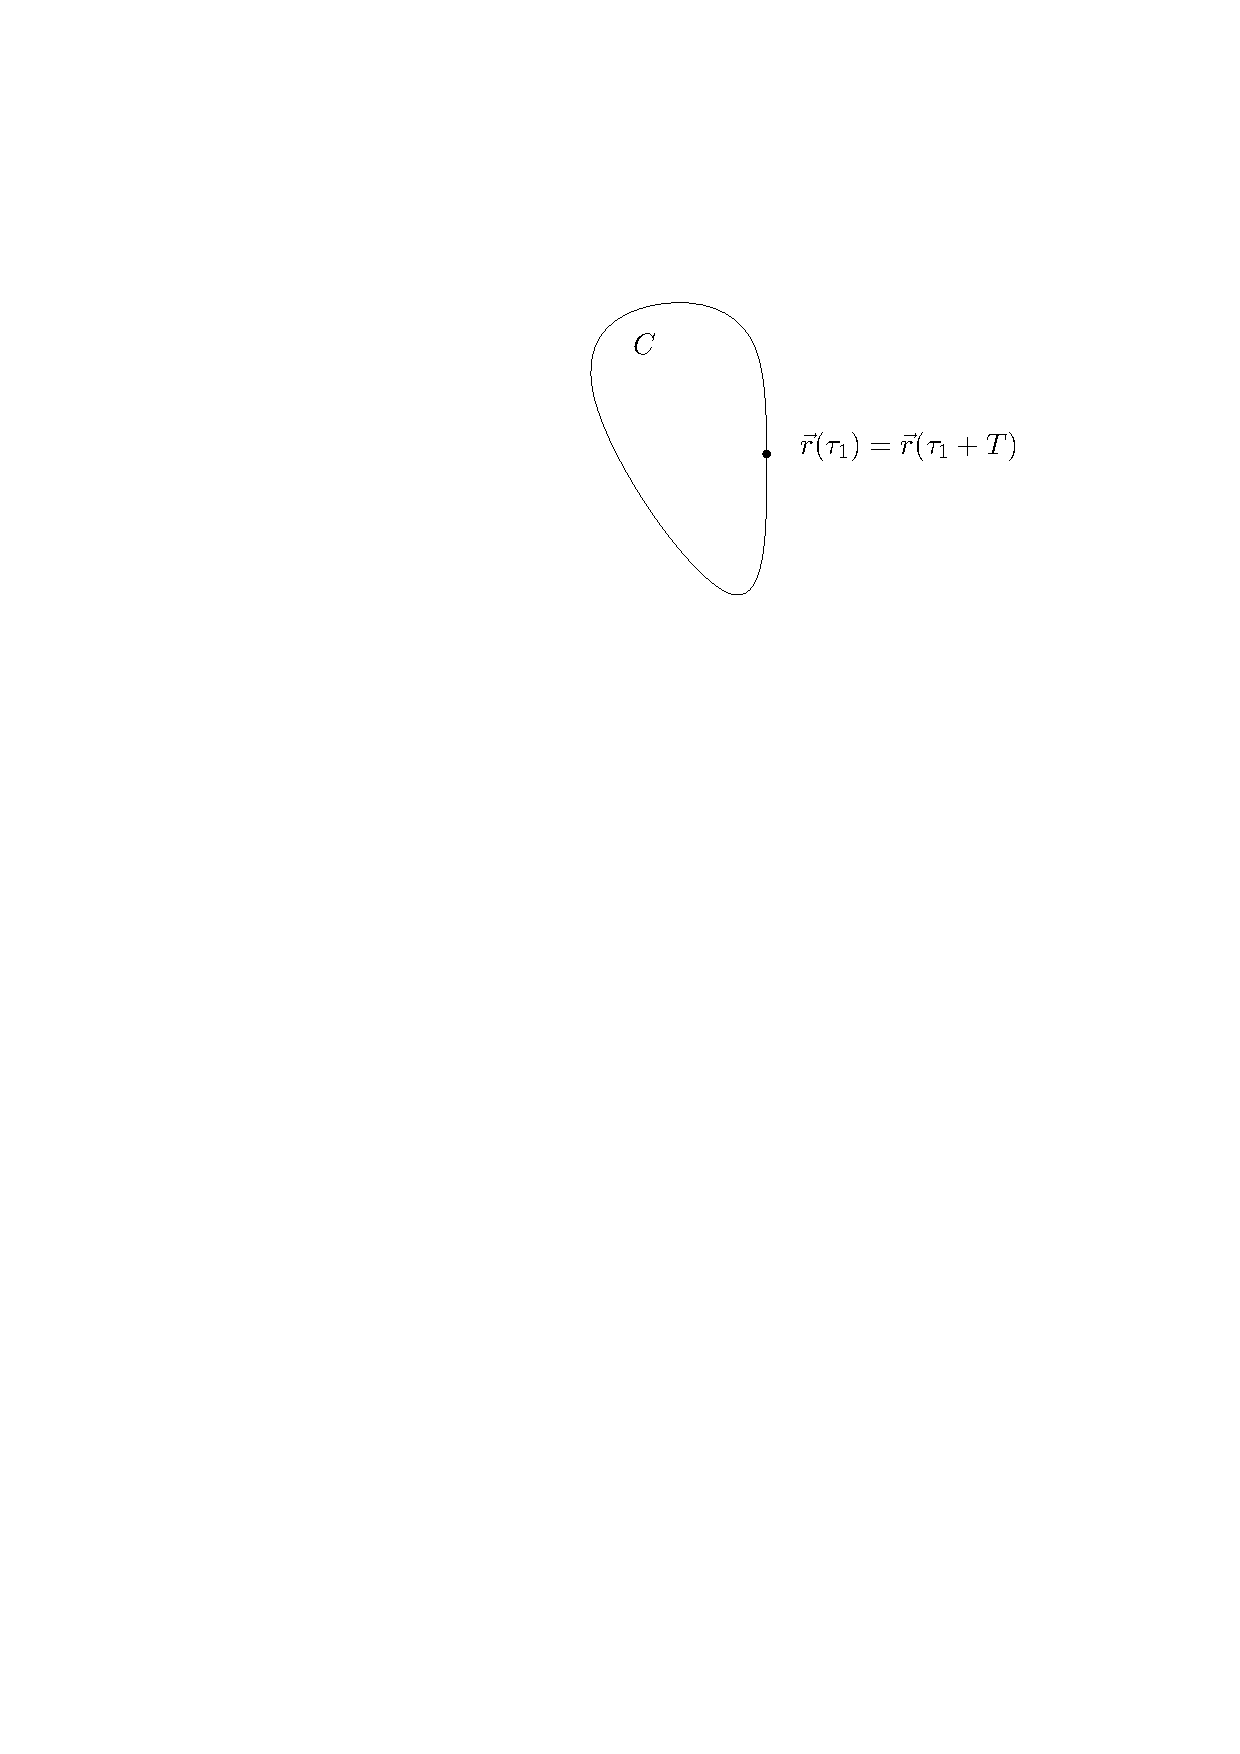
\includegraphics[width=0.4\linewidth]{fig/slutenkurva.pdf}}



Man skriver då integralen som
\begin{equation}
  \oint_C \vec{F} \cdot \mbox{d}\vec{r}.
\end{equation}

Det finns andra typer av linjeintegraler, till exempel
\begin{equation}
  \int \phi \mbox{d}\vec{r}, \quad \int \phi \mbox{d}s
\end{equation}
där $\phi$ är ett skalärt fält och $\mbox{d}s = | \mbox{d}\vec{r} | $. Samt
\begin{equation}
  \int \vec{F} \times \mbox{d}\vec{r}, \quad \int \vec{F} \mbox{d}s.
\end{equation}

\subsection{Studera räkneexempel:}
\begin{itemize}
\item Kurvintegral, cirkel 1

\item Kurvintegral, cirkel 2
\end{itemize}

\noindent
\subsection{Konservativa fält}
Om 
\begin{equation}
  \oint_C \vec{F} \cdot\mbox{d}\vec{r} = 0
\end{equation}
för varje sluten kurva $C$, så säges fältet $\vec{F}$ vara konservativt.  För ett konservativt fält $\vec{F}$ gäller att givet en fix startpunkt A och en fix slutpunkt B, så beror integralen
\begin{equation}
  \int_C \vec{F} \cdot\mbox{d}\vec{r}
\end{equation}
inte på valet av kurvan $C$ mellan dessa punkter.  Betrakta två kurvor $C_1$ och $C_2$ mellan A och B.  Då kan vi skapa en sluten kurva $C_0$ genom att först följa kurvan $C_1$ från A till B, och sedan kurvan $C_2$ baklänges, det vill säga i negativ riktning, tillbaka till A. Integralen över $C_0$ måste då vara 0, fast den integralen kan vi också skriva som
\begin{equation}
  \oint_{C_0} \vec{F} \cdot\mbox{d}\vec{r} = \int_{C_1} 
\vec{F} \cdot\mbox{d}\vec{r} - \int_{C_2} \vec{F} \cdot\mbox{d}\vec{r} = 0,
\end{equation}
ty integralen byter tecken om vi följer kurvan i \emph{fel} riktning. Nu följer det att 
\begin{equation}
  \int_{C_1} \vec{F} \cdot\mbox{d}\vec{r} = \int_{C_2} \vec{F} \cdot\mbox{d}
\vec{r}.
\end{equation}

\subsection{Studera räkneexempel:}
\begin{itemize}
\item Kurvintegral, fältstyrka
\end{itemize}

\noindent
\paragraph{Parametrisering av ytintegraler:}
Precis som man kan beräkna linjeintegralerna genom att parametrisera linjen längs vilken man integrerar kan man beräkna ytintegralerna genom att parametrisera ytan längs med vilken man integrerar.  Skillnaden är att genom att ytan är två-dimensionell så behöver man två parametrar. Antag att ortsvektorerna för punkterna på ytan kan skrivas som $\vec{r}(v,w)$ där $v$ och $w$ är våra parametrar.  Vi kan då bilda två tangentvektorer till ytan
\begin{equation}
  \frac{\partial \vec{r}}{\partial v} \quad \mathrm{och} \quad
\frac{\partial \vec{r}}{\partial w}.
\end{equation}
Förutsatt att dessa tangentvektorer inte är parallella, annars måste vi finna en ny parametrisering, kan vi bilda en normalvektor till ytan
\begin{equation}
  \frac{\partial \vec{r}}{\partial v} \times \frac{\partial \vec{r}}{\partial w}.
\end{equation}



% inline figure
\centerline{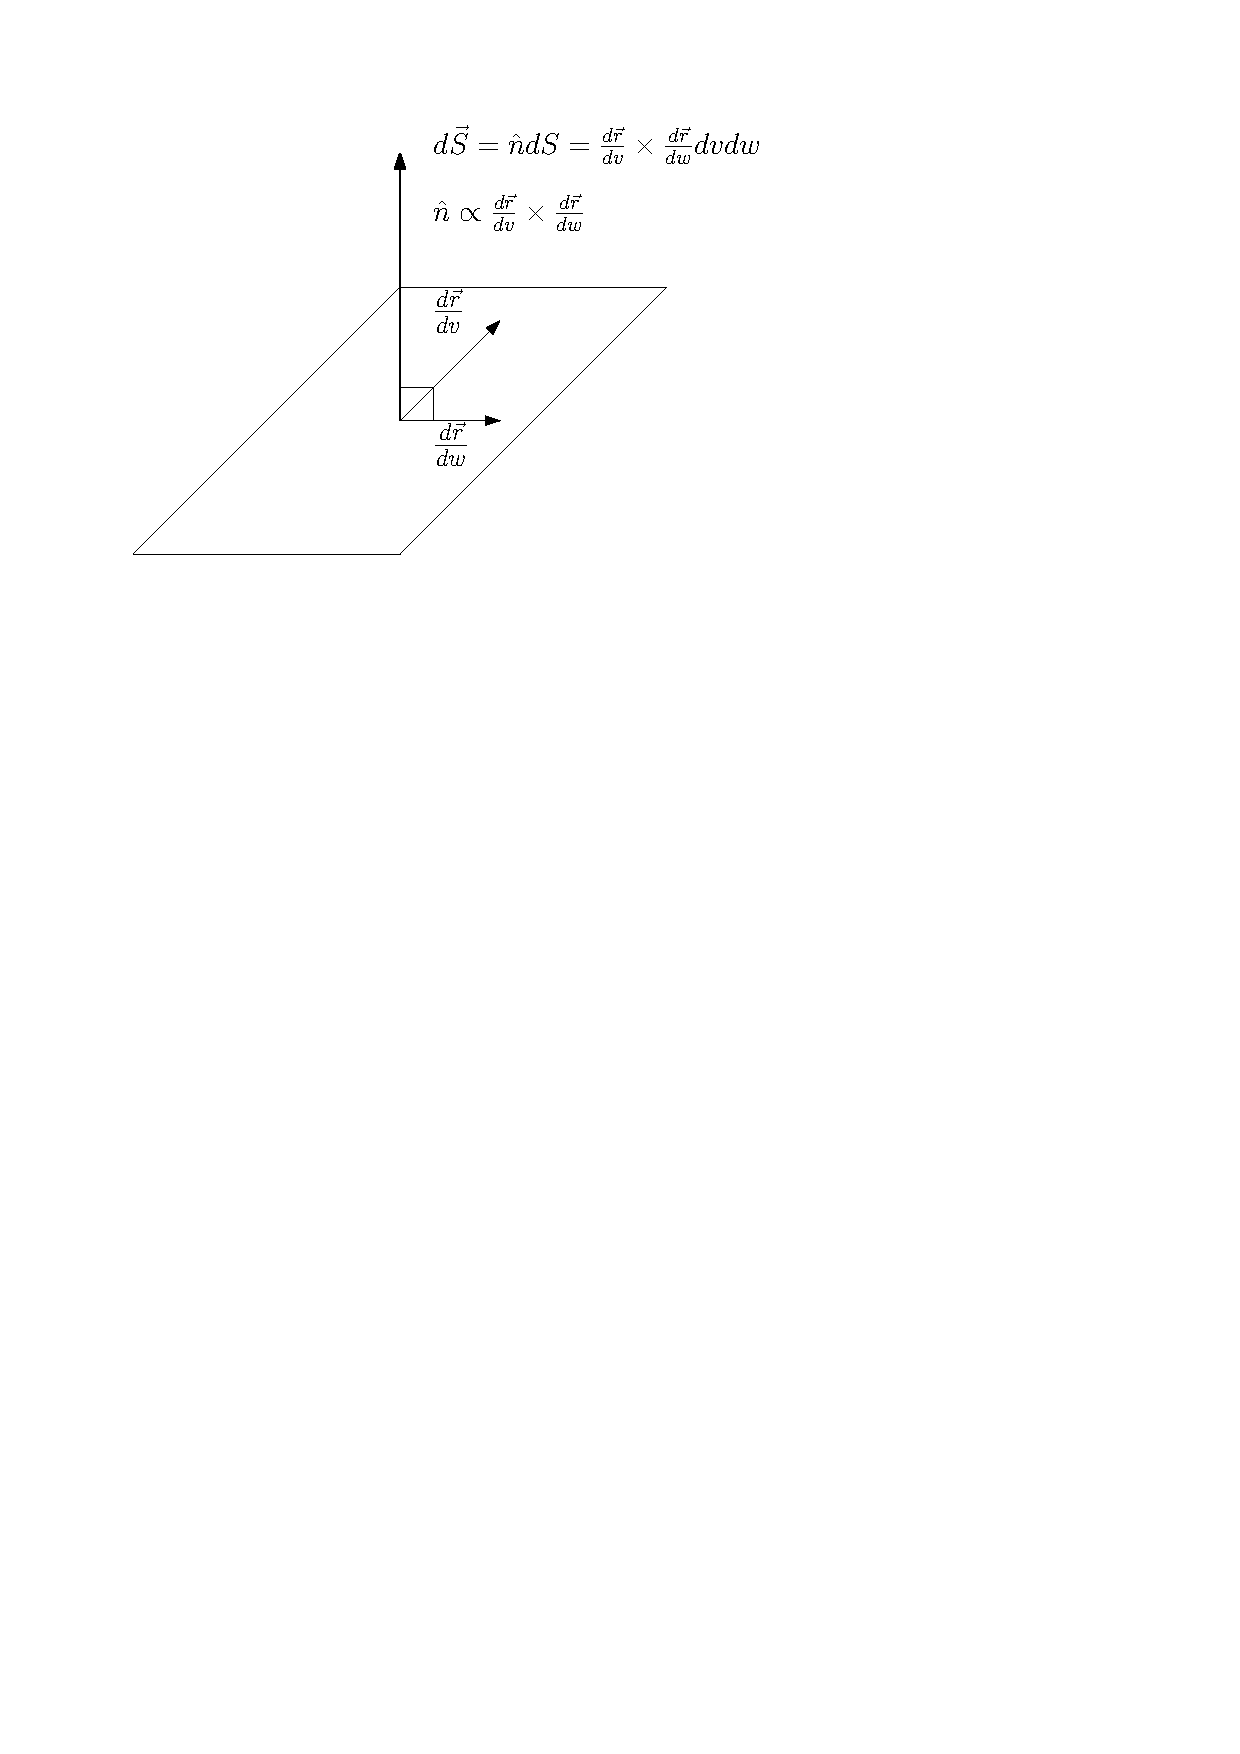
\includegraphics[width=0.6\linewidth]{fig/ytparametrisering.pdf}}



Analogt med hur vi tidigare uttryckte linjeintegralen med hjälp av vår parameter kan vi nu skriva ytintegralen som
\begin{equation}
  \int_S \vec{F} \cdot \mbox{d}\vec{S} = \int_S \vec{F} \cdot 
\frac{\partial \vec{r}}{\partial v} \times \frac{\partial \vec{r}}{\partial w}
\mbox{d}v \mbox{d}w,
\end{equation}
där $\mbox{d}\vec{S} = \hat{n} \mbox{d}S = \frac{\partial \vec{r}}{\partial v} \times \frac{\partial \vec{r}}{\partial w} \mbox{d}v \mbox{d}w$ är ytan på det parallellogram som spänns upp av de två tangentvektorerna. Normalvektorn uppfyller $|\hat{n}|=1$.

Allmänt skriver man ytintegraler över en yta $S$ (ofta använder man i de här sammanhangen $S$ för att beteckna en yta) som
\begin{equation}
  \int_S \vec{F} \cdot \mbox{d}\vec{S}.
\end{equation}
För att skilja dessa integraler från andra ytintegraler, som emellanåt förekommer, kallar man dem för normalytintegraler.

\subsection{Studera räkneexempel:}
\begin{itemize}
\item Cylinderyta
\end{itemize}

\noindent
\longinlinecomment{Comment 2}{ För resten av den här kursen kommer det ofta att vara lämpligt att på detta sätt beskriva arean av ett ytelement som en vektor.  En komplikation är förstås att en yta i allmänhet har två motsatta normalvektorer, och man måste därför ange vilken riktning som är positiv. Ytterligare en komplikation är att det finns ytor för vilka man inte kan definiera normalvektorn på ett kontinuerligt sätt över hela ytan, till exempel Möbius-bandet.  Vi skall inte befatta oss med sådana ytor här, utan begränsa oss till orienterbara ytor, ytor som har en insida och en utsida. }{ För resten av den }

Om ytan $S$ är sluten så skriver man
\begin{equation}
  \oint_S \vec{F} \cdot \mbox{d}\vec{S}.
\end{equation}
För slutna ytor definierar man den positiva riktningen som den som ges av en vektor som pekar ut från den inneslutna volymen.

Det finns också andra former av ytintegraler, vilka emellanåt används:
\begin{equation}
  \int_S \phi dS,
\end{equation}
där $\phi$ är en skalär, och vi i detta fall inte betraktar $S$ som en 
vektor.
\begin{equation}
  \int_S \phi d\vec{S}
\end{equation}
Skillnaden mot det första fallet är att $S$ här behandlas som en vektor.
\begin{equation}
  \int_S \vec{v} \times d\vec{S}
\end{equation}
där $\vec{v}$ är en vektorvärd funktion.


\paragraph{Parametrisering av volymintegraler.}
Det finns bara två möjliga sätt att volymintegrera ett fält. Med (det skalära) volymelementet $\mbox{d}V$
\begin{equation}
\int_V \phi \mbox{d}V,\quad \int_V \vec{F} \mbox{d}V.
\end{equation}
En parametrisering med $(u,v,w)$ ger att volymselementet blir volymen av parallellepipeden med sidorna $\frac{\partial \vec{r}}{\partial u} \mbox{d}u$, $\frac{\partial \vec{r}}{\partial v} \mbox{d}v$, $\frac{\partial \vec{r}}{\partial w} \mbox{d}w$ (som då måste vara linjärt oberoende). Denna volym är
\begin{equation}
\mbox{d}V = \left| \frac{\partial \vec{r}}{\partial u} \cdot \left( \frac{\partial \vec{r}}{\partial v} \times \frac{\partial \vec{r}}{\partial w} \right) \right| \mbox{d}u \mbox{d}v \mbox{d}w.
\end{equation}

\subsection{Integration med ortogonala kroklinjiga koordinater}

Från tidigare kapitel har vi 
\begin{equation}
d\vec{r} = \hat{e}_1 h_1 du_1 + \hat{e}_2 h_2 du_2 + \hat{e}_3 h_3 du_3
\end{equation}

Vidare ytelementet, t.ex. för en $u_1$-yta (dvs i $u_2 u_3$-planet):
\begin{align}
\mbox{d} S_1 &= h_2 h_3 \mbox{d}u_2 \mbox{d}u_3 \\
\mbox{d} \vec{S}_1 &= \pm \hat{e}_1 h_2 h_3 \mbox{d}u_2 \mbox{d}u_3 
\end{align}
vilket man t.ex. ser från 
\begin{equation}
\mbox{d} \vec{S}_1 = \frac{d\vec{r}}{du_2} \times \frac{d\vec{r}}{du_3} du_2 du_3
= \hat{e}_1 h_2 h_3 \mbox{d}u_2 \mbox{d}u_3 
\end{equation}

Volymelement:
\begin{equation}
\mbox{d} V = h_1 h_2 h_3 \mbox{d}u_1 \mbox{d}u_2 \mbox{d}u_3.
\end{equation}

Med ett vektorfält $\vec{F}$ som tecknas i det kroklinjiga koordinatsystemet $\vec{F} = F_1 \hat{e}_1 + F_2 \hat{e}_2 + F_3 \hat{e}_3$ får vi t.ex.
\begin{align}
\int_{C_1} \vec{F} \cdot d\vec{r} &= \int_{C_1} F_1 h_1 du_1 \\
\int_{S_1} \vec{F} \cdot d\vec{S}_1 &= \int_{S_1} F_1 h_2 h_3 du_2 du_3 \\
\int_V \vec{F} dV &= \int_V \vec{F} h_1 h_2 h_3 du_a du_2 du_3,
\end{align}
där $C_1$ är en kurva längs $u_1$-riktningen och $S_1$ är en $u_1$-yta.

\subsection{Räkneexempel: Linjeintegraler}

\paragraph{Exempel: Kurvintegral, cirkel 1.}
---------------------------------------------

Beräkna integralen $\oint_C \phi d\vec{r}$ där $\phi = \phi_0$ (konstant) och kurvan $C$ beskriver en cirkel i xy-planet med radie $a$ och centrum i origo som genomlöps medurs.

\begin{itemize}
\item Notera att svaret kommer att bli en vektor.

\item Parametrisera kurvan (notera riktningen): $\vec{r}(\tau) = x(\tau)\hat{x} + y(\tau)\hat{y} = a \sin\omega\tau \hat{x} + a \cos\omega\tau \hat{y}$ med $\tau \in [0,2\pi/\omega]$.

\item Vi inkluderar konstanten $\omega$ för att illustrera att det finns ett oändligt antal parametriseringar och att svaret inte kan bero på detta.

\item Förskjutningsvektorn $d\vec{r} = \hat{x} \frac{dx}{d\tau}d\tau + \hat{y} \frac{dy}{d\tau}d\tau$.
\end{itemize}

\noindent
Den parametriserade kurvintegralen blir
\begin{equation}
\oint_C \phi d\vec{r} = \phi_0 \oint_0^{2\pi/\omega} \left[
\hat{x} a \omega\cos\omega\tau - \hat{y} a \omega\sin\omega\tau \right] d\tau = 0
\end{equation}

---------------------------------------------

\paragraph{Exempel: Kurvintegral, cirkel 2.}
---------------------------------------------

Beräkna integralen $\oint_C \phi dr$ där $\phi = \phi_0$ (konstant) och kurvan $C$ beskriver en cirkel i xy-planet med radie $a$ och centrum i origo som genomlöps medurs.

\begin{itemize}
\item Notera att svaret kommer att bli en skalär.

\item Lite eftertanke ger att svaret borde bli $\phi_0 2 \pi a$, dvs den konstanta potentialen gånger omkretsen på cirkeln.

\item Bågelementet blir $dr = |d\vec{r}| = \sqrt{\left( \frac{dx}{d\tau} \right)^2 d\tau^2 + \left( \frac{dy}{d\tau} \right)^2 d\tau^2 } = a \omega d\tau$
\end{itemize}

\noindent
Den parametriserade kurvintegralen blir
\begin{equation}
\oint_C \phi ds = \phi_0 a \omega \oint_0^{2\pi/\omega}  d\tau = \phi_0 2 \pi a 
\end{equation}

---------------------------------------------

\paragraph{Exempel: Kurvintegral, fältstyrka.}
---------------------------------------------

Betrakta kurvintegralen $\int_C \vec{A} \cdot d\vec{r}$ där $\vec{A} = -\nabla \phi$, dvs en fältstyrka.
\begin{itemize}
\item Det betyder att $\int_C \vec{A} \cdot d\vec{r} = -\int_C \nabla{\phi} \cdot d\vec{r}$.

\item Kom ihåg att $\nabla\phi \cdot d\vec{r} = d\phi$.

\item Alltså $\int_C \vec{A} \cdot d\vec{r} = -\int_{\phi_1}^{\phi_2} d{\phi} = \phi_1 - \phi_2$.
\end{itemize}

\noindent
Dvs kurvintegralen av en fältstyrka är oberoende av vägen $C$ utan beror bara på potentialens värden i start- och slutpunkterna.

---------------------------------------------
\paragraph{Exempel: Kraft och arbete.}
---------------------------------------------

En partikel rör sig längs en bana C, som ges av $\vec{r}(t)$, under inverkan av en kraft $\vec{F}(\vec{r})$.  Vi vill då beräkna arbetet som kraften utövar på partikeln.  Mellan punkterna $\vec{r}$ och $\vec{r}+\mbox{d}\vec{r}$ så är arbetet
\begin{equation}
  \mbox{d}W = \vec{F}\cdot \mbox{d}\vec{r}.
\end{equation}
Vi kan då beräkna arbetet längs hela kurvan genom att beräkna integralen
\begin{equation}
  W = \int_C \vec{F}\cdot \mbox{d}\vec{r}.
\end{equation}
Denna integral är ett exempel på en linjeintegral (kurvintegral). Vi kan skriva
\begin{equation}
  W = \int_C \vec{F} \cdot \frac{\mbox{d}\vec{r}}{\mbox{d}t} \mbox{d}t = \int P \mbox{d}t,
\end{equation}
där $P$ är effekten.

---------------------------------------------

\paragraph{Exempel: Konservativ kraft och arbete.}
-----------------------------------------

En elektron rör sig längs banan $y = \frac{x^2}{H}$ från $(0,0)$ till $(L,L^2/H)$ under inverkan av en elektrostatisk kraft $\vec{F} = e E_0\hat{y}$.  Beräkna det arbete som kraften utför på elektronen.

\emph{Lösning 1:}  Arbetet ges av integralen
\begin{equation}
  \int_C eE_0 \hat{y} \cdot \mbox{d}\vec{r},
\end{equation}
där $C$ är den kurva som elektronen följer.  Vi kan nu använda koordinaten $x$ för att parametrisera vår kurva och skriver kurvan som $\vec{r}(x) = (x, x^2/H)$.  Då gäller att
\begin{equation}
  \frac{\mbox{d}\vec{r}}{\mbox{d}x} = \left(1,\frac{2x}{H}\right).
\end{equation}
Vi kan nu beräkna arbetet ur
\begin{equation}
  \int_C eE_0 \hat{y} \cdot \mbox{d}\vec{r} = \int_0^LeE_0 \hat{y} \cdot
\frac{\mbox{d}\vec{r}}{\mbox{d}x} \mbox{d}x = \int_0^LeE_0 \frac{2x}{H} 
\mbox{d}x = \frac{eE_0}{H} \left[x^2\right]_0^L = \frac{e E_0 L^2}{H}.
\end{equation}

\emph{Lösning 2:}  Elektrostatiska krafter är konservativa, så vi kan ersätta kurvan med två räta linjer, en $C_1$ som går från $(0,0)$ till $(L,0)$ och är parallell med $x$-axeln, och en kurva $C_2$ som går från $(L,0)$ till $(L,L^2/H)$ och är parallell med $y$-axeln. Arbetet kan nu skrivas som
\begin{equation}
   \int_C eE_0 \hat{y} \cdot \mbox{d}r = \int_{C_1} eE_0 
\hat{y} \cdot \mbox{d}r + \int_{C_2} eE_0 \hat{y} \cdot \mbox{d}r.
\end{equation}
Eftersom kraften överallt är ortogonal mot kurvan $C_1$ följer att 
integralen längs med $C_1$ måste vara noll, så det återstår bara att beräkna
\begin{equation}
\int_{C_2} eE_0 \hat{y} \cdot \mbox{d} \vec{r} = \int_{C_2} 
e E_0 \hat{y} \cdot \hat{y} \mbox{d}r = e E_0 \int_{C_2} \mbox{d}r.
\end{equation}
Den sista integralen ger nu längden på kurvan $C_2$, vilken är $L^2/H$,
så arbetet blir till slut
\begin{equation}
  \frac{e E_0 L^2}{H}.
\end{equation}

---------------------------------------------

\paragraph{Exempel: Parametriserad 3d-kurva.}
---------------------------------------------

Beräkna integralen av $\vec{u} = (xy, z^2, x)$ längs med kurvan 
\begin{equation}
\left\{\begin{array}{lcl}
x & = & 1+t\\
y & = & 0\\
z & = & t^2\\
\end{array}\right. 
\end{equation}
där $0 \le t \le 3$.  

Vi beräknar då först 
\begin{equation}
  \frac{\mbox{d}\vec{r}}{\mbox{d}t} = (1, 0, 2t).
\end{equation}
Vektorfältet uttryckt i $t$ är
\begin{equation}
  \vec{u} = \left(\left(1+t\right) \cdot 0, t^4, 1+t\right) = 
\left(0,t^4,1+t\right).
\end{equation}
Skalärprodukten mellan vektorerna är
\begin{equation}
  \left(0,t^4,1+t\right) \cdot \left(1,0,2t\right) = 2t + 2t^2.
\end{equation}
Integralen blir
\begin{equation}
  \int_0^3 \left(2t+2t^2\right)\mbox{d}t = 
\left[t^2 + \frac{2t^3}{3}\right]_0^3 = 9 + 18 = 27.
\end{equation}

---------------------------------------------

\subsection{Räkneexempel: Ytintegraler}

\paragraph{Exempel: Flöde genom yta.}
--------------------------------------------- 

En vätska med densiteten $\rho$ och hastigheten $\vec{u}$ strömmar parallellt genom ett rör med tvärsnittsarean $A$.  Flödet av vätska genom röret (det vill säga kg vätska som per sekund strömmar genom röret är då $\rho u A$.  

Vad händer då om vätskans  hastighet $\vec{u}$ beror på avståndet $r$ från rörets symmetriaxel?  I så fall får vi definiera en flödestäthet $\rho u(r)$ så att flödet genom ett ytelement $dS$ blir $\rho u(r)dS$. Om vi tar $dS$ som en ring med centrum i symmetriaxeln och med en tjocklek d$r$ så är d$A = 2\pi r$d$r$ och det totala flödet genom röret blir
\begin{equation}
  \int \rho u( r ) dS = \int_0^R \rho u ( r ) 2 \pi r
dr,
\end{equation}
där $R$ är rörets radie.

För att nu ytterligare komplicera det hela och verkligen blanda in vektorerna så antar vi att vätskan strömmar genom en tvärsnittsarea $dS$, vilken inte är vinkelrät mot vätskans strömningshastighet $\vec{u}$.  Vi antar att vinkeln mellan normalvektorn $\vec{n}$ till ytan $dS$ och vätskans hastighet $\vec{u}$ är $\theta$.  Då blir flödet genom ytan $dS$
\begin{equation}
  \rho u dS \cos \theta.
\end{equation}
Om vi nu väljer att definiera en vektor $d\vec{S}$ för ett ytelement med storleken $dS$ och riktningen $\vec{n}$, så ser vi att vi kan skriva flödet som
\begin{equation}
  \rho \vec{u} \cdot d\vec{S},
\end{equation}
där $\rho \vec{u}$ kan kallas för en massflödestäthet (jämför med en strömtäthet för flöde av elektrisk laddning).

Vi kan nu skriva vätskeflödet genom en godtycklig yta $A$ som
\begin{equation}
  \int_A \rho \vec{u} \cdot d\vec{S},
\end{equation}
vilket är ett typiskt exempel på en ytintegral.

---------------------------------------------

\paragraph{Exempel: Cylinderyta.}
---------------------------------------------

Beräkna ytintegralen av fältet $\vec{u} = (x,z,-y)$ över cylinderytan $x^2 + y^2 = 1$ mellan $z = 0$ och $z = 1$.  Vi kan då beskriva punkterna på ytan genom deras $z$-koordinat och vinkeln $\varphi$ som ortsvektorn bildar med $\hat{x}$-vektorn.  Det vill säga $\vec{r} = (\cos\varphi , \sin\varphi , z)$, och tangentvektorerna blir
\begin{equation}
  \frac{\mbox{d}\vec{r}}{\mbox{d} \varphi} = \left(-\sin\varphi , \cos \varphi ,
0\right)
\end{equation}
och
\begin{equation}
  \frac{\mbox{d}\vec{r}}{\mbox{d}z} = \left(0,0,1\right).
\end{equation}
Normalvektorn blir
\begin{equation}
  \frac{\mbox{d}\vec{r}}{\mbox{d} \varphi} \times 
\frac{\mbox{d}\vec{r}}{\mbox{d}z} = \left(\cos\varphi , \sin \varphi, 0\right).
\end{equation}
Vi kan sedan beräkna integralen som
\begin{align}
  \int_S \vec{u} \cdot \mbox{d}\vec{S} &= \int_0^1\int_0^{2\pi} \left(\cos\varphi,
z, -\sin\varphi\right) \cdot \left(\cos\varphi, \sin \varphi, 0\right)
\mbox{d}\varphi \mbox{d}z \nonumber \\
&= \int_0^1\int_0^{2\pi} \left(\cos^2\varphi + z
\sin\varphi\right) \mbox{d}\varphi\mbox{d}z \nonumber \\
&= \int_0^1 \int_0^{2\pi} \left(
\frac{1}{2} + \frac{1}{2}\cos 2\varphi + z\sin\varphi\right) \mbox{d}\varphi
\mbox{d}z \nonumber \\
&= \int_0^1 \left[\frac{1}{2}\varphi + \frac{1}{4}\sin2\varphi - z
\cos\varphi\right]_0^{2\pi} \mbox{d}z = \int_0^1 \pi \mbox{d}z = \pi.
\end{align}

---------------------------------------------




% ------------------- end of main content ---------------


% #ifdef PREAMBLE
\printindex

\end{document}
% #endif

